\documentclass[titlepage]{article}

\usepackage[utf8]{inputenc}
\usepackage{natbib}
\usepackage{graphicx}
\usepackage{caption}
\usepackage{subcaption}
\usepackage{hyperref}
\usepackage{listings}
\usepackage[export]{adjustbox}
\usepackage{indentfirst}
\usepackage[section]{placeins}
\usepackage[a4paper]{geometry}
\usepackage{minted}
\usepackage{amsmath}
\usepackage{siunitx}
\usepackage{fancyhdr}

\title{Discrete Fourier Transform}

\author{
  Diogo \\ Dionatan \\ Gabriel \\ Vincent 
}

\date{October 2017}

\begin{document}
\maketitle

\section{Introduction}


When processing a signal (an image, audio, etc) it has to be sampled at a finite number of points since one cannot compute data in a continuous manner. It usually turns out to be much more useful to store information about the frequency domain of our data (a plane wave, for example, is represented by a Dirac's delta). Thus it is more efficient to transmit data about the frequency spectrum.  This is done by applying a Fourier transform to a signal and later reconstructing it at the destination by applying the inverse Fourier transform. Furthermore real signals cannot in general be described by a smooth function that can be easily described in closed-form so we have to resort to discretizing it and extracting information from it from its frequency spectrum. The continuous Fourier transform is given by:

$$\hat{f}(\omega) = \frac{1}{\sqrt{\pi}}\int_{-\infty}^{+\infty}dxf(x)e^{-i\omega x}$$

And its inverse by:

$$f(x) = \frac{1}{\sqrt{\pi}}\int_{-\infty}^{+\infty}dx\hat{f}(\omega)e^{i\omega x}$$

To deal with the aforementioned scenario we need a discrete version of it:
$$\hat{f_n} = \frac{1}{N}\sum_{k=0}^{N-1}\Delta xf_k(x)e^{-i n x_k}\quad n \in {0,1,\dots,N-1}$$

\section{Discrete Fourier Transform}

Assume $f(x)$ is a periodic function in the interval $[0,2\pi]$ notice that it can always be made to be periodic by extending exact copies of $f(x), x \in [0,2\pi]$ throughout the domain $(-\infty,+\infty)$. But it is a bit messier to prove the case where the interval is arbitrary so we stick with $[0, 2\pi]$ for simplicity's sake.
Also suppose that $f(x)$ is sampled at $N$ points over the interval $[0,2\pi]$. It is important here that the sampling is made at linearly spaced points for the argument to work, that is, the kth sample point is given by:
$$x_k = \frac{2\pi k}{N}$$

The discrete Fourier transform is the set of coefficients of a complex trigonometric polynomial that interpolates $f(x)$ at the linearly spaced $x_k$ points. 
So one needs to find the coefficients $c_n$ of the interpolating polinomial:

$$f_k = \sum_{n=0}^{N-1} c_ne^{i n x_k}\quad k \in {0,1,\dots,N-1}$$

The strategy here relies on using Fourier's trick: multiply by an orthogonal  function and sum over all values, exploit the orthogonality to kill off a summation and end up with an expression for the coefficient $c_n$. Thus:

$$\sum_{k=0}^{N-1} f_ke^{-i m x_k} = \sum_{k=0}^{N-1} e^{-i m x_k}\sum_{n=0}^{N-1} c_ne^{i n x_k}$$

Rearranging the summations:

$$\sum_{k=0}^{N-1} f_ke^{-i m x_k} = \sum_{n=0}^{N-1} c_n\sum_{k=0}^{N-1}  e^{i (n-m) x_k}$$

Now the last summation can be broken down into two cases, the first where $n = m$:

$$\sum_{k=0}^{N-1} e^{i 0 x_k} = \sum_{k=0}^{N-1} 1 = N$$

And the other where $n\neq m$. To evaluate this case, first substitute for $x_k$:

$$\sum_{k=0}^{N-1}  e^{i (n-m) x_k} = \sum_{k=0}^{N-1}  e^{i (n-m) \frac{2\pi k}{N}} $$

Then let $r = e^{i 2\pi (n-m)}$ and use the finite geometric sum:

$$\sum_{k=0}^{N-1}  e^{i (n-m) \frac{2\pi k}{N}} = \sum_{k=0}^{N-1}r^k  = S$$
$$S = 1 + r + r^2+\dots+r^{N-1} $$
$$rS = r + r^2+r^3+\dots+r^{N-1}+r^{N} $$
$$S-rS = 1-r^{N}$$
$$S = \frac{1-r^{N}}{1-r}$$

Recall that $n$ and $m$ are integers belonging to ${0,1,\dots,N-1}$ which makes 
$$r = e^{i 2\pi (n-m)} = e^{i 2\pi\times\mbox{an integer}}  = 1$$

And the geometric sum in turn:

$$S = \frac{1-r^{N}}{1-r} = 0$$

Which converges to 0 since $r^N$ approaches 0 much faster than $r^1$ does

Therefore we conclude that $\sum_{k=0}^{N-1}  e^{i (n-m) x_k}$ is either $N$ for $n=m$ or $0$ otherwise. Using this information:

$$\sum_{k=0}^{N-1} f_ke^{-i m x_k} = \sum_{n=0}^{N-1} c_nN\delta_{nm} = c_mN$$

The coefficients are then given by:

$$c_n = \frac{1}{N} \sum_{k=0}^{N-1} f_ke^{-i n x_k}$$

The discrete Fourier transform is defined as:

$$\hat{f_n} = Nc_n = \sum_{k=0}^{N-1} f_ke^{-i n x_k}$$

\subsection{Implementation}

It is quite straightforward to put together a simple implementation of the Discrete Fourier Transform, below is one done in Mathematica which reflects exactly the formula deduced above:

\begin{minted}{Mathematica}
dft[f_List] :=  With[{t = Length[f]},  
	Table[Total@Table[f[[k + 1]] Exp[-((I 2 Pi n k)/t)], {k, 0, t - 1}], {n, 0,t - 1}]]
(*sample input*)
dft[{0, 1, 4, 9}]
(*result*)
{14., -4. + 8. I, -6., -4. - 8. I}
\end{minted}

\section{Fast Fourier Transform}

The direct computation of the discrete Fourier transform requires $n*k$ operations which is of the order $O(N^2)$. This means that for a mere 1000 points a million such operations need be performed. The fast Fourier transform is a clever algorithm that reduces the same problem to order O(N log N). It works by halving the problem into even and odd indices recursively until a problem of size 2 is reached and then summing back all the pieces to give the answer.

For this to work the number of sample points must be of the form $2^p$. So let $N=2^p$ and $M=\frac{N}{2}$. Start from the discrete Fourier transform. To simplify notation let $w_N = e^{-\frac{2\pi i}{N}}$ thus:

$$\hat{f_n} = \sum_{k=0}^{N-1} f_ke^{-\frac{i 2\pi n k}{N}}= \sum_{k=0}^{N-1} f_kw^{nk}_N$$

Split the summation into odd and even indices both of size $M=\frac{N}{2}$:

$$\hat{f_n} = \sum_{k=0}^{M-1} f_{2k}w^{n2k}_N + \sum_{k=0}^{M-1} f_{2k+1}w^{n(2k+1)}_N$$

Since $(w_N)^2 = w_M$:

$$w^{n2k}_N = (w^{nk}_N)^2 = e^{-\frac{2\pi i}{N/2}}=e^{-\frac{2\pi i}{M}}=w^{nk}_M$$

It reduces to the following:

$$\hat{f_n} = \sum_{k=0}^{M} f_{2k}w^{nk}_M + w_M^n\sum_{k=0}^{M} f_{2k+1}w^{nk}_M$$

The full matrix operation is $\hat{f} = W*f$ where W is the matrix of components $w^{nk}$ where $n$ indexes rows and $k$ does columns.

So our formula is incomplete because $n$ goes com $0$ to $2M$ while we have halved the matrix $W$ from $W_N$ to $W_M$ which cannot be multiplied by a vector $f$ of dimensions $n\times 1$. So to account for that we treat the case where $n$ is of the form $n + M$ like this:

$$\hat{f}_{n+M} = \sum_{k=0}^{M} f_{2k}w^{(n+M)k}_M + w_M^{n+M}\sum_{k=0}^{M} f_{2k+1}w^{(n+M)k}_M$$

Upon noticing that:

$$w^M_M = e^{-\frac{2\pi iM}{M}}=1$$
$$w^M_N = e^{-\frac{2\pi iM}{N}}=e^{-\frac{2\pi iN}{2N}}=e^{-i\pi}=-1$$

$$\hat{f}_{n+M} = \sum_{k=0}^M f_{2k}w^{nk}_M - w^n_N\sum_{k=0}^M f_{2k+1}w^{nk}_M$$

We get the same formula with a sign change.

We continue on dividing each summation into two summations for even and odd indices and keep doing it recursively until we reach two summations of two terms each. When all this is done we perform the sums and multiplications of the resulting, completely expanded, expression and we get the discrete Fourier components just as before using the direct discrete transform.

\subsection{Implementation}

Such an algorithm of recursive nature is ideally suited for functional languages, we chose to make a loose implementation in Haskell:

\begin{minted}{Haskell}
import Data.List
import Data.Complex

--two simple functions that extract even/odd-indexed elements from a list:
odds [] = []
odds [x] = []
odds (e1:e2:xs) = e2 : odds xs

evens [] = []
evens [x] = []
evens (e1:e2:xs) = e1 : evens xs

--this is the factor that multiplies the odd summation in the fft algorithm, 
--kept separated for readability
f xs n = exp $ -(0:+2*pi)*n / genericLength xs

--if the function is called with just two elements x and y:
ffti [x,y] n = x + y * (exp $ -(0:+pi)*n)
--if the function is called with a list bigger than 2 applying the function again 
--but splitting it into two summations of even and odd indexed elements:
ffti xs n = ffti (evens xs) n + f xs n * ffti (odds xs) n

--consume the input list 
fft xs [] = []
fft xs (y:ys) = (ffti xs y):(fft xs ys)

--input
fft [0, 1, 4, 9] [0,1,2,3]

--result (where the notation :+ means complex number in Haskell)
[14.0 :+ 0.0,(-4.000000000000002) :+ 7.999999999999999, 
(-6.0) :+ (-2.449293598294706e-15),(-3.999999999999995) :+ (-8.000000000000002)]

--or rounding:
[14.0 :+ 0.0,
-4.0 :+ 8.0, 
-6.0 :+ 0.0, 
-4.0 :+ -8.0)]
\end{minted}

Haskell being a pure functional language most readily lends itself to this task, but it can be done in an also simple fashion in semi-functional languages like Mathematica:

\begin{minted}{Mathematica}
(*treat the special case of a list containing two elements*)
fft[{x_, y_}, n_] := x + y Exp[-I Pi n ]
(*otherwise split the list into even- and odd-indexed elements*)
(*and apply the function recursively*)
fft[f_List, n_] :=                fft[Downsample[f, 2, 1], n] + 
    Exp[-((I 2 Pi n )/Length[f])] fft[Downsample[f, 2, 2], n]
(*the above handles a particular f_n, below handle all n's*)
fft[f_List] := Table[fft[f, n] // N, {n, 0, Length[f] - 1}]
(*sample input*)
fft[{0, 1, 4, 9}]
(*result*)
{14., -4. + 8. I, -6., -4. - 8. I}
\end{minted}

Both implementations were tested against a few different inputs and gave the same results as the fft function from MATLAB and Python. But Wolfram Mathematica's Fourier function differs by a constant factor because we considered our $x_k$ points sample at $\frac{2\pi k}{N}$ and Mathematica considers a shorter interval of $\frac{\pi k}{N}$

\section{Aliasing}

A quick word of caution against sampling at too few points. One could sample a signal with a frequency of 1 at -7,-6,...0,1,...7 and get the points below:

\begin{figure}[ht]
\centering
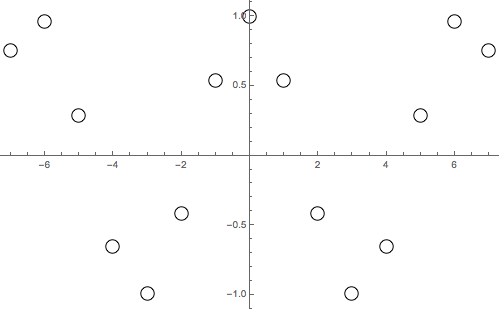
\includegraphics[scale = 0.5, center]{images/alias1.png}
\caption{Alias 1}
\label{fig:2d}
\end{figure}
\FloatBarrier

Which one might guess might correspond to the function $cos(t)$:

\begin{figure}[ht]
\centering
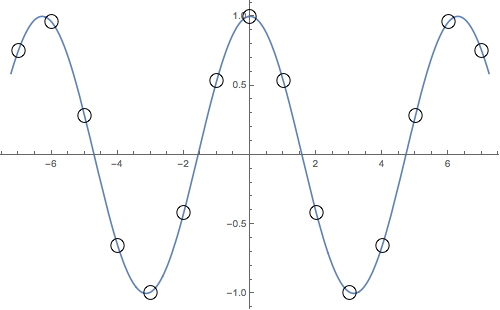
\includegraphics[scale = 0.5, center]{images/alias2.png}
\caption{Alias 1}
\label{fig:2d}
\end{figure}
\FloatBarrier

However we may be the case that our function actually has higher frequency $cos((2\pi-1)t)$ and our meager sample rate of 1 was unable to capture it:

\begin{figure}[ht]
\centering
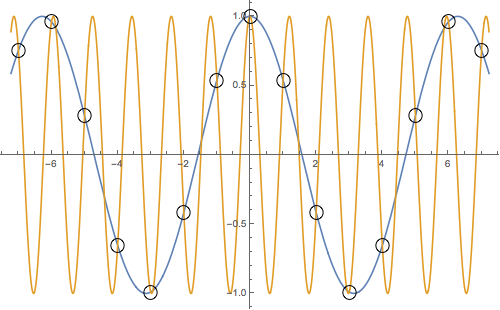
\includegraphics[scale = 0.5, center]{images/alias3.png}
\caption{Alias 1}
\label{fig:2d}
\end{figure}
\FloatBarrier

So a good rule is to follow Nyquist's sampling theorem which states (proves) that the sampling rate must be at least twice the highest frequency one expects to encounter in sampling a signal.

\section{Application: Textbook examples}
\subsection{Gaussian}
A common textbook application of the fourier transform is to apply it on a gaussian function:

\begin{figure}[ht]
\centering
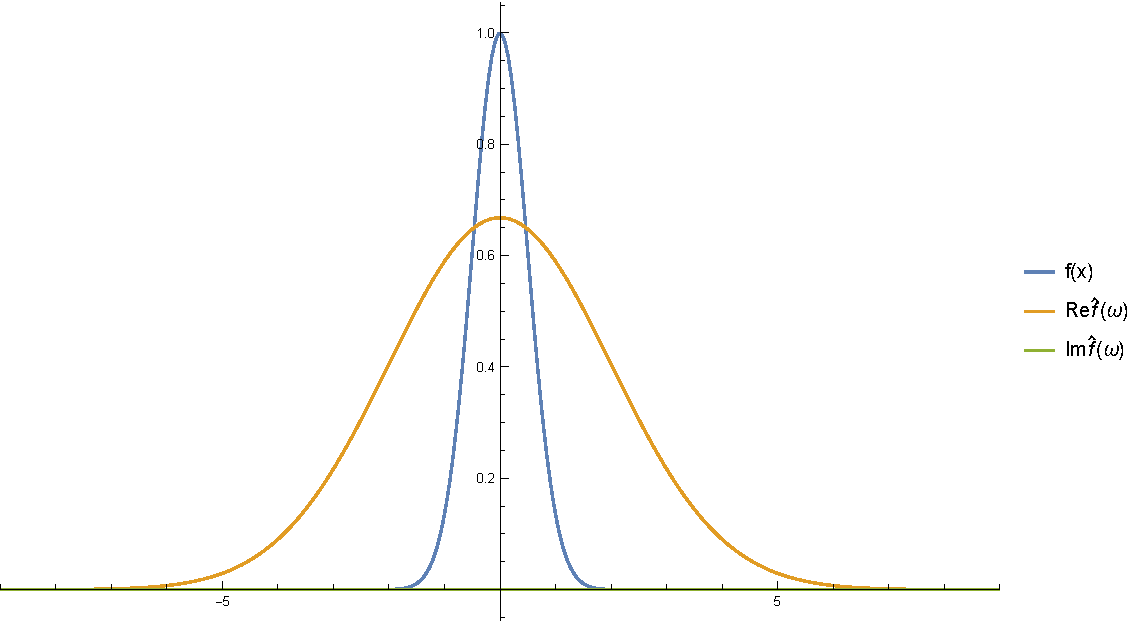
\includegraphics[scale=0.8,center]{images/gaussian1.pdf}
\caption{Alias 1}
\label{fig:2d}
\end{figure}
\FloatBarrier

One notices that the Fourier transform is also a gaussian but since f(x) is narrow the Fourier transform will correspondingly be broad which is a well know result in math that relates to the uncertainty principle in physics.

We can make the gaussian broader to get a correspondingly narrow transform:

\begin{figure}[ht]
\centering
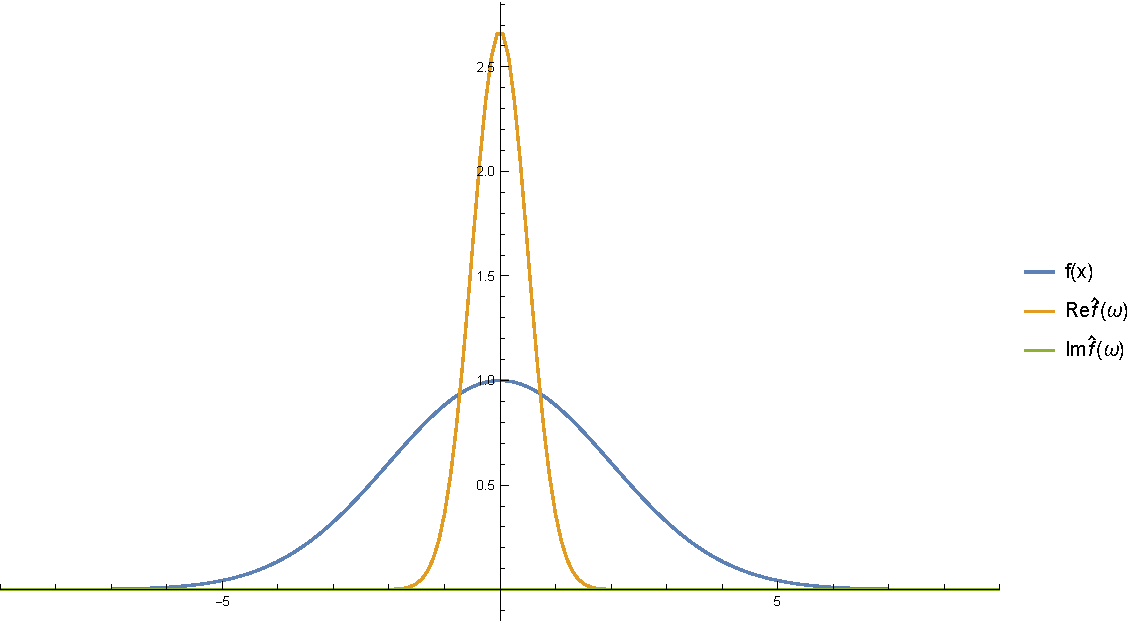
\includegraphics[scale=0.8,center]{images/gaussian2.pdf}
\caption{Alias 1}
\label{fig:2d}
\end{figure}
\FloatBarrier

Also the gaussian centered at 0 has no imaginary component. That changes if we nudge it to the right:

\begin{figure}[ht]
\centering
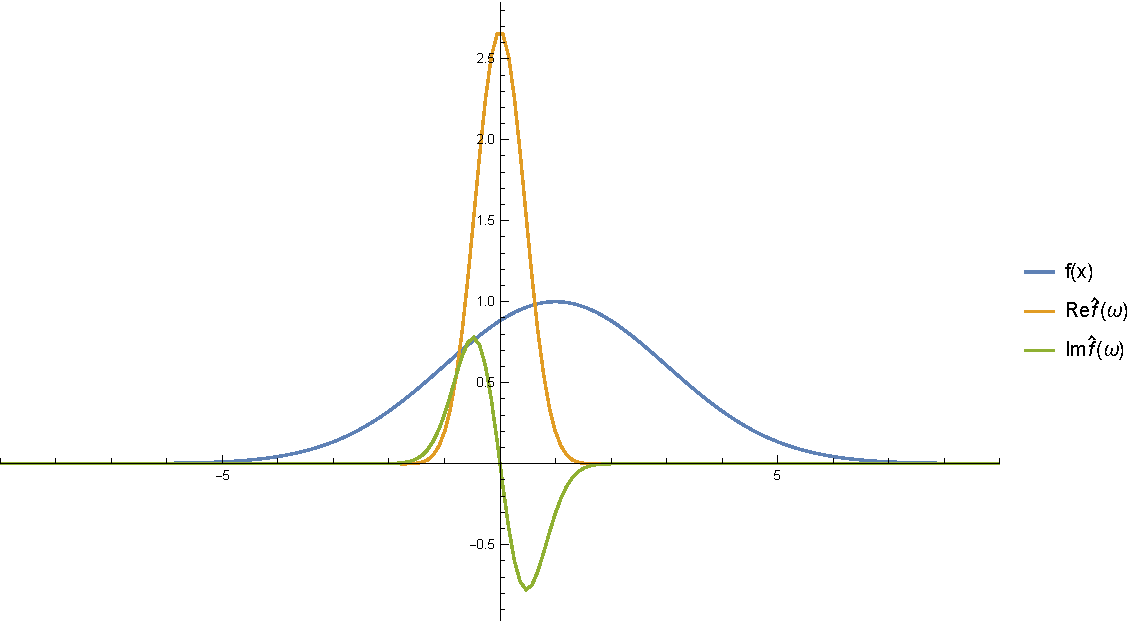
\includegraphics[scale=0.8,center]{images/gaussian3.pdf}
\caption{Alias 1}
\label{fig:2d}
\end{figure}
\FloatBarrier

\subsection{Code}
Unfortunately the dead simple textbook code we started with cannot handle an arbitrary sample rate and neither an arbitrary starting value of x. So we changed the code to handle those hurdles:
\begin{minted}{Mathematica}
(*an alternative and completely equivalent way to compute the dft is commented in the middle*)
(*it makes the operations matrix-wise, matlab-style instead of "nth element-wise"*)
dft[ts_List, fs_List] := (
  l = Length[ts]; 
  dt = Abs@ts[[2]] - Abs@ts[[1]] // Abs;
  w0 = -Pi/dt;
  ws = Array[# &, l, {-Abs@w0, Abs@w0}];
  dw = Abs@ws[[2]] - Abs@ws[[1]] // Abs;
  t0 = ts[[1]] ;
  gs = Table[
     Total@Table[
       fs[[k + 1]] Exp[-I (w0 + n*dw) (t0 + k*dt)], {k, 0, 
        l - 1}], {n, 0, l - 1}]/Sqrt[l - 1];
  (*gs = Exp[-\[ImaginaryI]*Outer[Times,ws,ts]].fs/Sqrt[l-1];*)
  
  grpts = Riffle[ws // N, Re@gs // N]~Partition~2;
  gipts = Riffle[ws // N, Im@gs // N]~Partition~2;
  fpts = Riffle[ts // N, fs // N]~Partition~2;
  {fpts, grpts, gipts}
  (*ListLinePlot[{fpts,gpts},PlotRange\[Rule]Full,
  ImageSize\[Rule]Large]*)
  )
(*generating a gaussian with 2^10 points from t=-30 to t=30*)
gaussian[t_, m_, s_] := Exp[-((t - m)^2/(2 s^2))];
t0 = -30;
l = 2^10;
(*MATLAB linspace equivalent*)
ts = Array[# &, l, {-Abs@t0, Abs@t0}];
(*computing*)
data = dft[ts, Table[gaussian[t, 0, 0.5], {t, ts}]];
(*plotting the results*)
ListLinePlot[data, PlotRange -> {{-9, 9}, Full}]
\end{minted}

\subsection{Harmonic Oscillator}

Another common example plotted below:

\begin{figure}[ht]
\centering
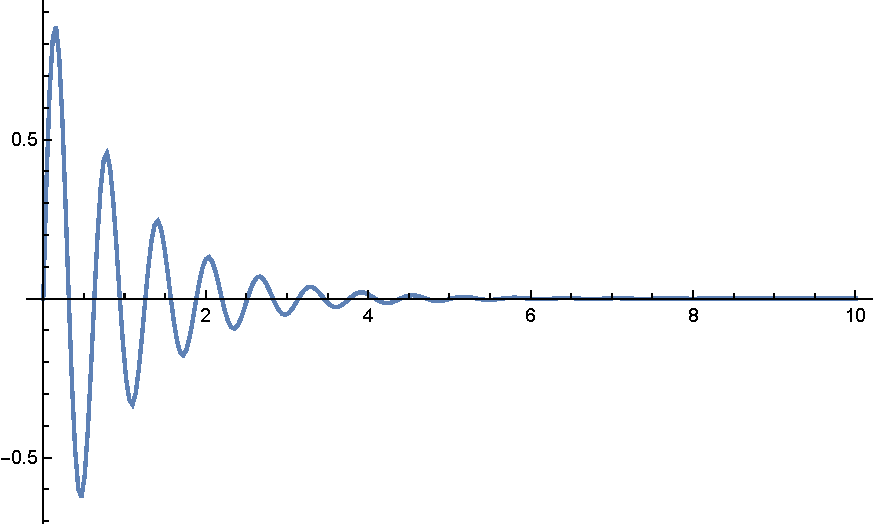
\includegraphics[scale=0.8,center]{images/osch.pdf}
\caption{Alias 1}
\label{fig:2d}
\end{figure}
\FloatBarrier

Its real Fourier transform:

\begin{figure}[ht]
\centering
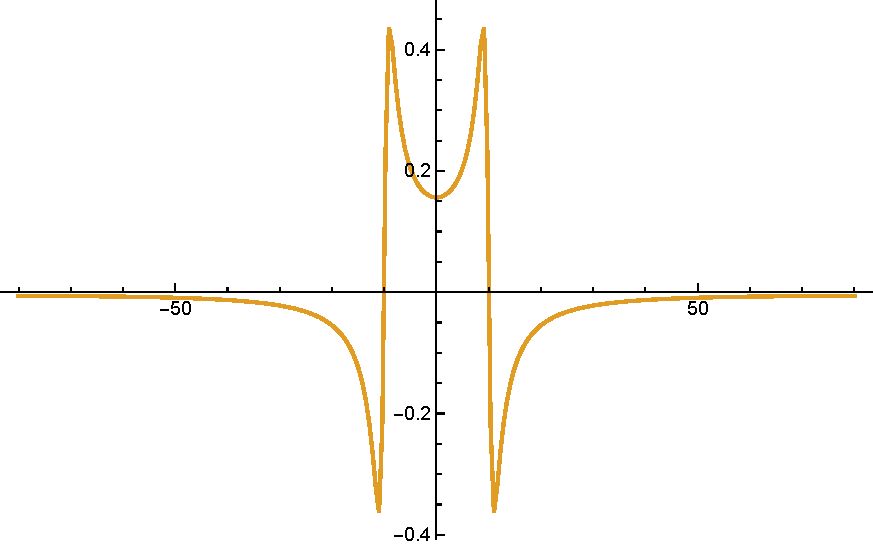
\includegraphics[scale=0.8,center]{images/oschre.pdf}
\caption{Alias 1}
\label{fig:2d}
\end{figure}
\FloatBarrier

And from its imaginary Fourier transform we can see the harmonic oscillator's resonant frequency, in this case about $\pm 10Hz$

\begin{figure}[ht]
\centering
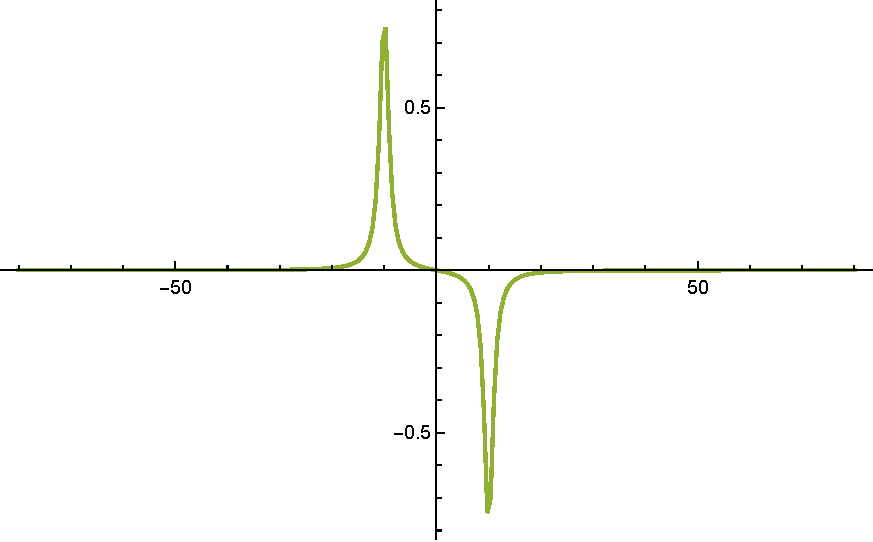
\includegraphics[scale=0.8,center]{images/oschim.pdf}
\caption{Alias 1}
\label{fig:2d}
\end{figure}
\FloatBarrier

\subsection{Code}
The code just builds upon what has been done for the gaussian previously:

\begin{minted}{Mathematica}
osc[t_] := Sin[10 t] Exp[-t];
l = 2^8;
ts = Array[# &, l, {0, 10}];
data = dft[ts, osc /@ ts];
Column@Table[ListLinePlot[data[[i]]], {i, 1, 3, 1}];
\end{minted}

\section{Application: Quantum Particle Through Potential Barrier}

An interesting application of the Fast Fourier Transform is to simulate the dynamics of a particle trying to overcome a potential barrier.
Classically if the potential is higher in energy than the particle's total energy it is impossible for it to cross such a barrier. Now for a particle 
described by quantum mechanics there's a small but non-zero probability of the particle crossing the barrier (tunnelling through it)
Below we reproduce the work done by Jake (at) where he produces an animation of the physical situation described above.
I have extensively modified his code in order to both understand and change its parameters. So I dumbed down his clearly written and explained, over-300-lines code 
to a terse and densely packed 60-liner but easily modifiable to my purposes.
The core of the code is the time\_step function that advances the particle. We can see that the leap-frog technique is used by advancing $\psi(x)$ by half a step
then computing $\psi(k)$ from the (fast) Fourier transform of $\psi(x)$. Then evolve $\psi(k)$ a step and compute $\psi(x)$ by the inverse Fourier transform of $\psi(k)$. Finally a full step is performed for $\psi(x)$.

\begin{minted}{Python}
def time_step():
    global t, psi_mod_x, psi_mod_k, t_max
    psi_mod_x *= x_evolve_half
    for i in range(N_steps):
        psi_mod_k = fft(psi_mod_x)
        psi_mod_k *= k_evolve
        psi_mod_x = ifft(psi_mod_k)
        psi_mod_x *= x_evolve_half*x_evolve_half
    psi_mod_k = fft(psi_mod_x)
    t += dt * N_steps
    t_max = t_max - 1
\end{minted}

The rest of the code is entirely bootstrapping: defining the potential, constants, initial and boundary conditions.

This python code processes the time evolution of each point of the interval [-100,100] and it runs 50 times for each time step: a lot of processing!
This can be done reasonably fast using the fast Fourier transform.

The results are written to files and read in Mathematica to do the animation. What follows are frames from animations using a few different potentials.

\subsection{Square potential}

Any introductory course in quantum mechanics solves Schr\"odinger's equation for the square potential barrier. Below are a few frames from the animation produced from the code above. We are seeing a probability wave propagating through both real and momentum space

\begin{figure}[ht]
\centering
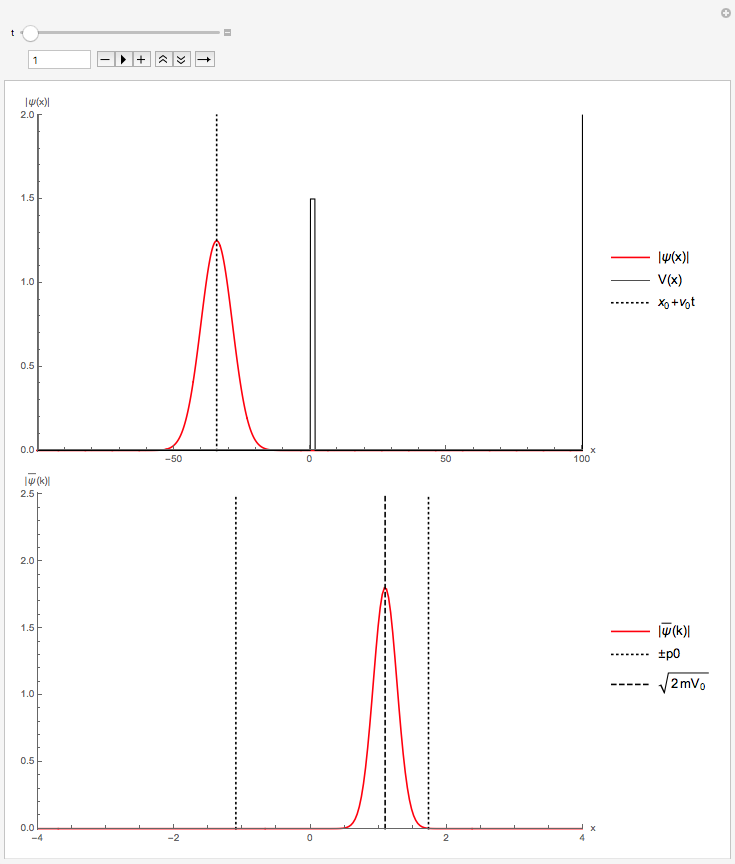
\includegraphics[scale=0.5,center]{images/square1.png}
\caption{Initial setting}
\label{fig:2d}
\end{figure}
\FloatBarrier

\begin{figure}[ht]
\centering
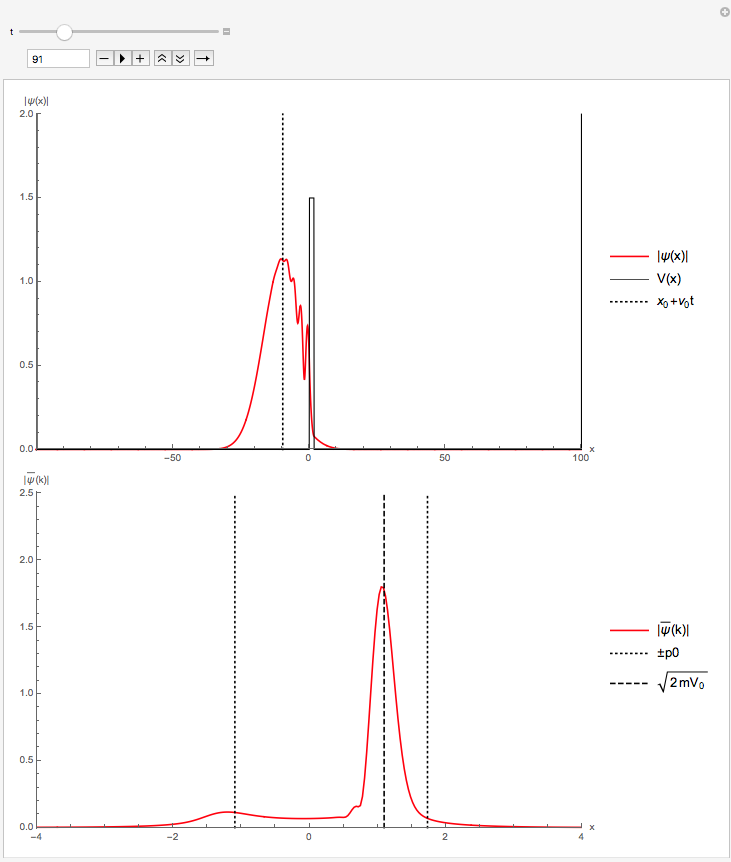
\includegraphics[scale=0.5,center]{images/square2.png}
\caption{Middle of animation}
\label{fig:2d}
\end{figure}
\FloatBarrier

It is clear that a portion of the probability makes its way to the other side!

\begin{figure}[ht]
\centering
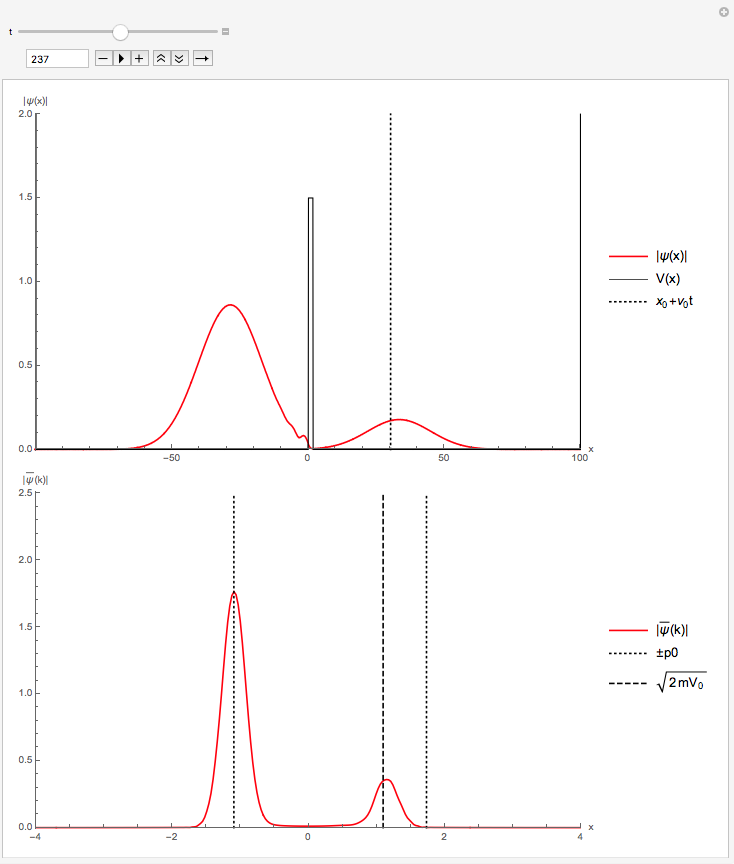
\includegraphics[scale=0.5,center]{images/square3.png}
\caption{Near the end of the animation}
\label{fig:2d}
\end{figure}
\FloatBarrier

\subsection{Triangular potential}

If the quantum mechanics professor is a bit bold he may dabble in solving the triangular potential:

\begin{figure}[ht]
\centering
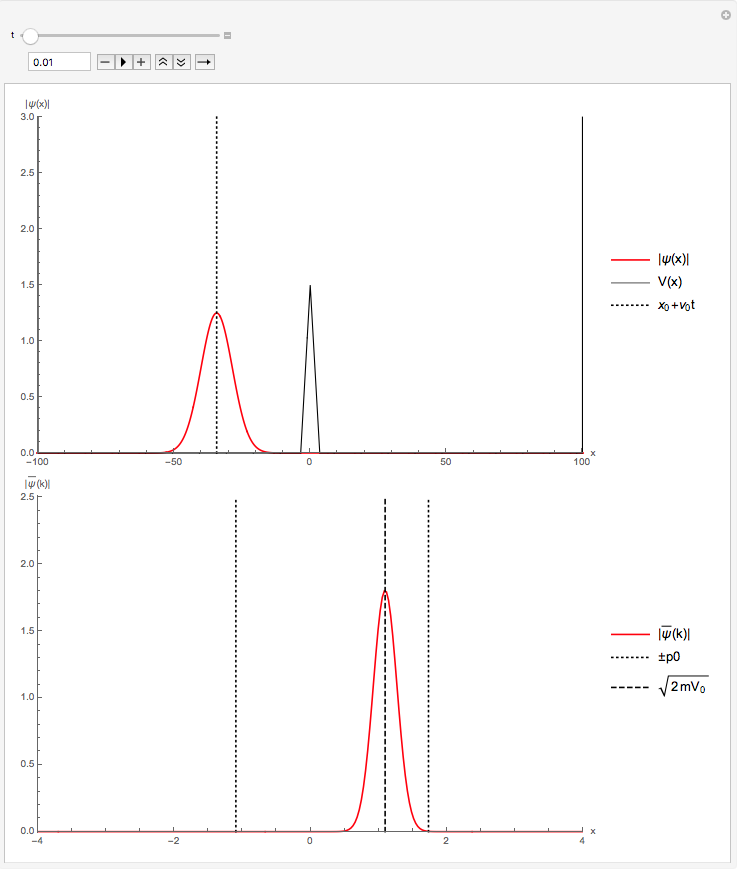
\includegraphics[scale=0.5,center]{images/triangular1.png}
\caption{Initial setting}
\label{fig:2d}
\end{figure}
\FloatBarrier

\begin{figure}[ht]
\centering
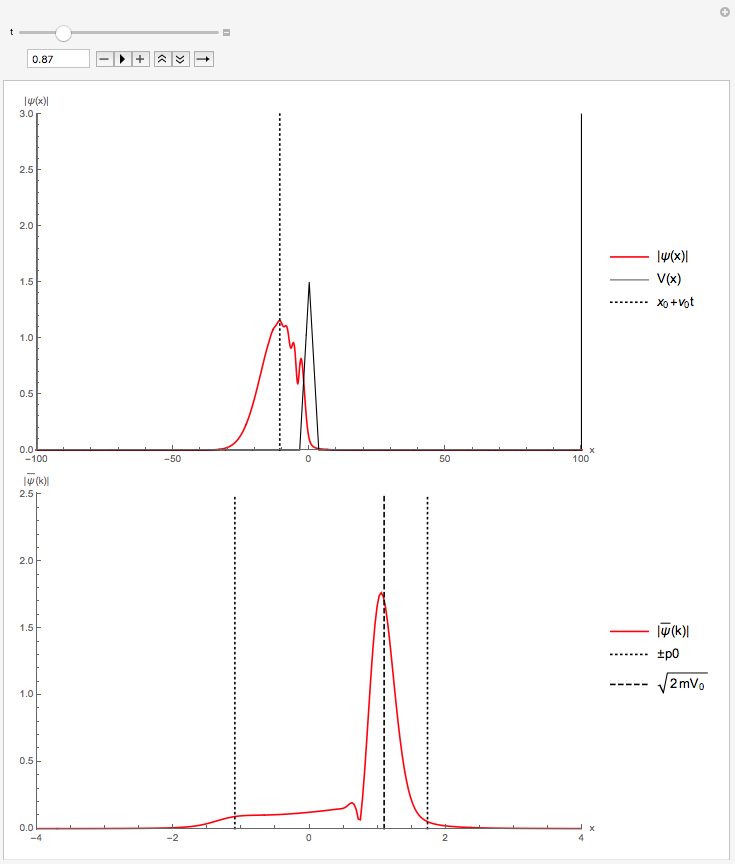
\includegraphics[scale=0.5,center]{images/triangular2.png}
\caption{Middle of animation}
\label{fig:2d}
\end{figure}
\FloatBarrier

A little probability also gets through

\begin{figure}[ht]
\centering
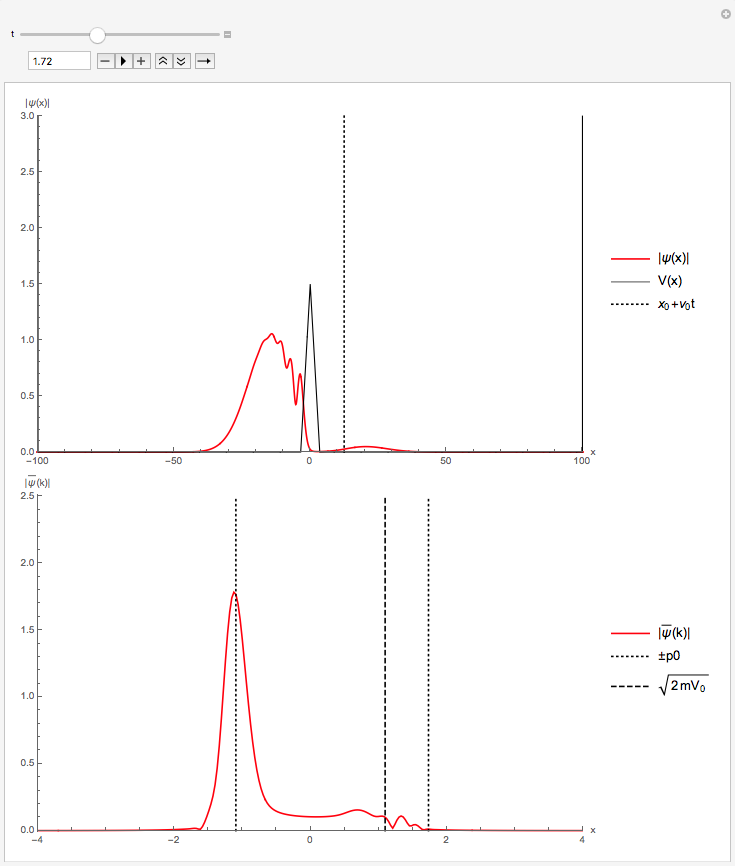
\includegraphics[scale=0.5,center]{images/triangular3.png}
\caption{Near the end of the animation}
\label{fig:2d}
\end{figure}
\FloatBarrier

\subsection{What if}

But if you're anything like me you might have imagined what would happen if the potential had a crazy shape, in my case, I thought what if we had a batman potential!

\begin{figure}[ht]
\centering
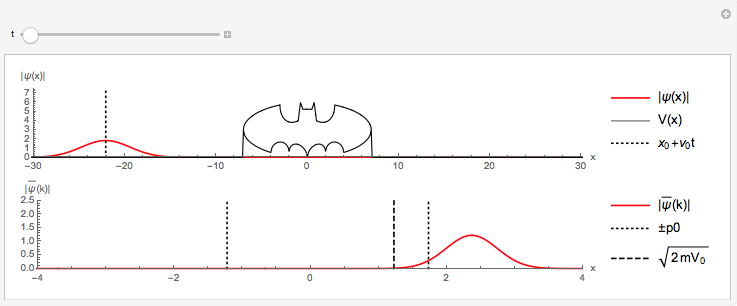
\includegraphics[scale=0.5,center]{images/batman1.png}
\caption{Initial setting}
\label{fig:2d}
\end{figure}
\FloatBarrier

\begin{figure}[ht]
\centering
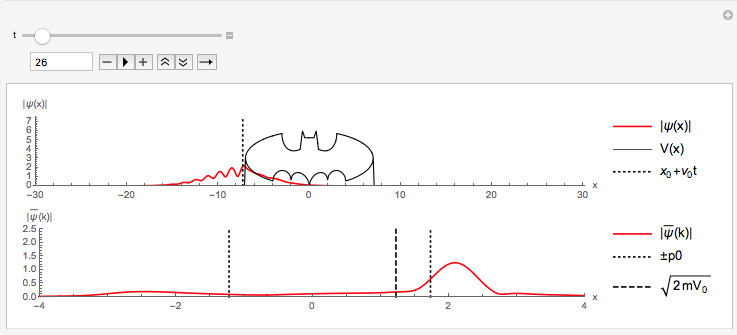
\includegraphics[scale=0.5,center]{images/batman2.png}
\caption{Middle of animation}
\label{fig:2d}
\end{figure}
\FloatBarrier

\begin{figure}[ht]
\centering
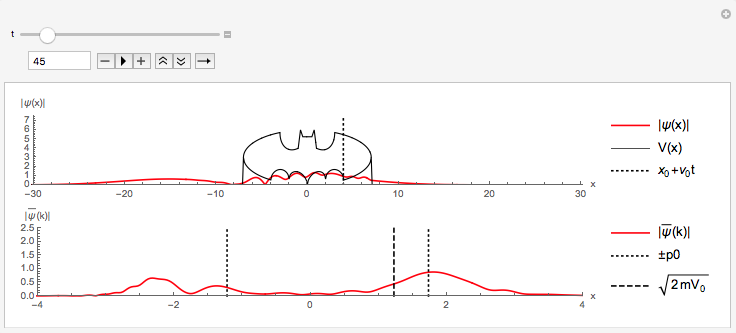
\includegraphics[scale=0.5,center]{images/batman3.png}
\caption{Near the end of the animation}
\label{fig:2d}
\end{figure}
\FloatBarrier

If we ignore the aspect ratio of the picture and do instead an automatic scaling the image becomes bigger and it's easier to see details

\begin{figure}[ht]
\centering
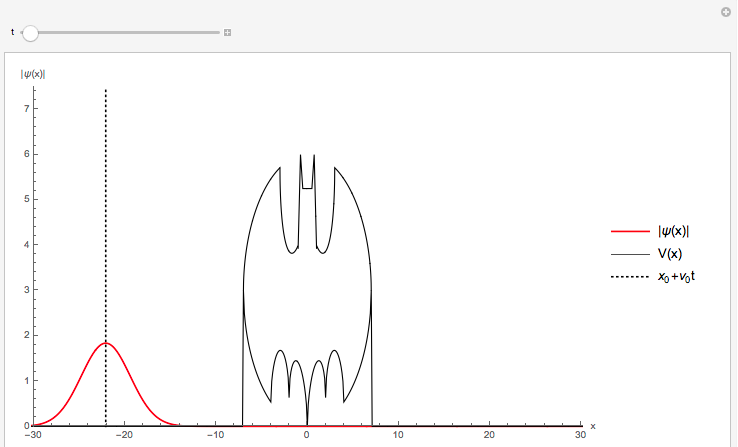
\includegraphics[scale=0.5,center]{images/batmanbig1.png}
\caption{Alias 1}
\label{fig:2d}
\end{figure}
\FloatBarrier

\begin{figure}[ht]
\centering
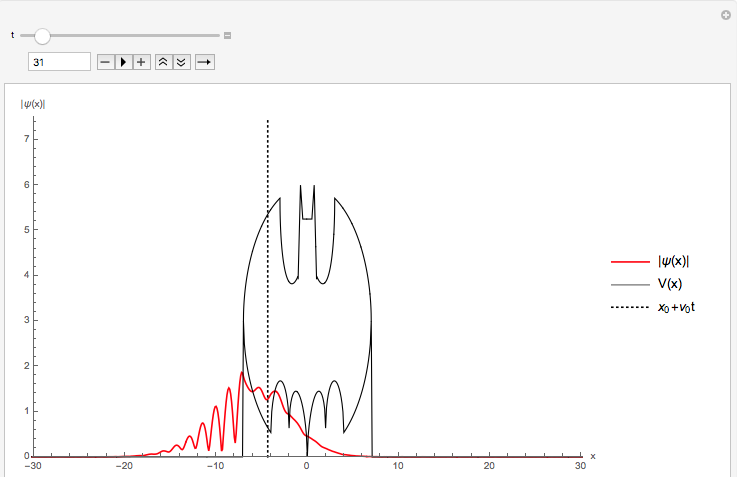
\includegraphics[scale=0.5,center]{images/batmanbig2.png}
\caption{Alias 1}
\label{fig:2d}
\end{figure}
\FloatBarrier

\begin{figure}[ht]
\centering
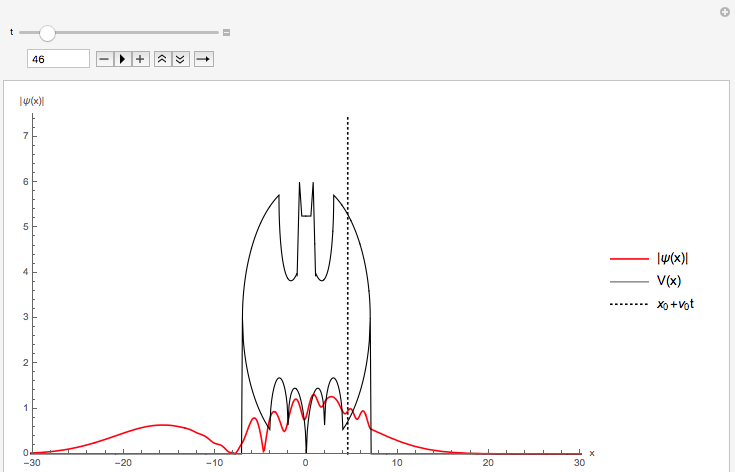
\includegraphics[scale=0.5,center]{images/batmanbig3.png}
\caption{Alias 1}
\label{fig:2d}
\end{figure}
\FloatBarrier

\end{document}
